\section{Evaluation}
\label{sec:evaluation}

We provide and evalutation based on two different models, following two different goals. First, we want to compare EMFFrag to its related world from the software modeling world using a software models. Secondly, we want to show the influence of different granularity of fragmentation on different performance parameters.

All experiments were conducted on a \markus{TODO}. All measures were repeated at least 20 times, and all present results are respective averages.

\subsection{Grabats -- Actual Software Models}

In this section, we will evaluate our approach to EMF/XMI, CDO, and Morsa. To cover as many use cases as possible, we will look at four abstract parameters: execution time of creating/manipulating, accessing complete models, accessing specific parts of models (query), and memory usage.

\begin{figure}[ht]
\begin{minipage}[b]{0.48\linewidth}
\centering
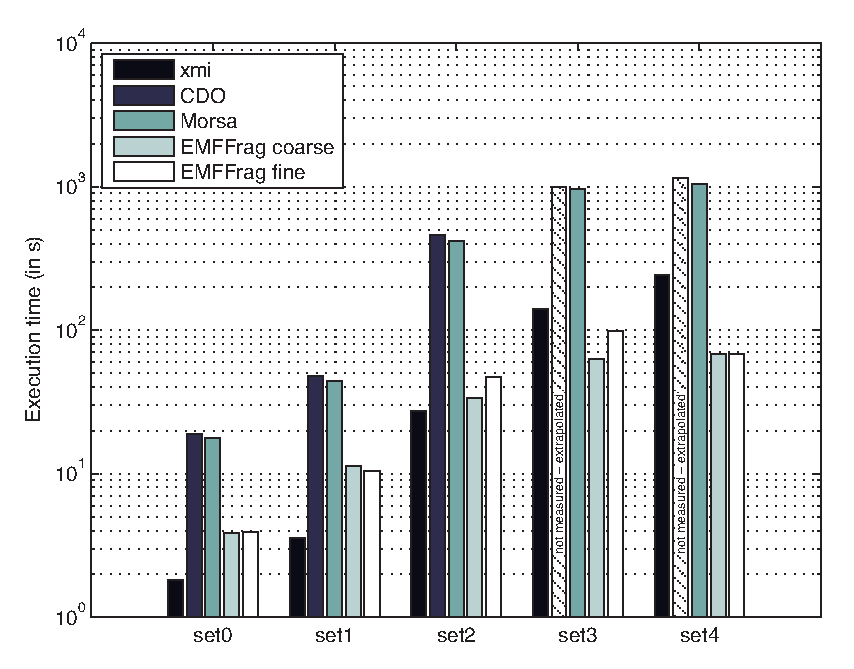
\includegraphics[width=\linewidth]{figures/grabatsTraverseTimeExtra}
\caption{Execution time for traversing the different Grabats models with the different persistence solutions.}
\label{fig:grabatsTraverseTime}
\end{minipage}
\hspace{0.02\linewidth}
\begin{minipage}[b]{0.48\linewidth}
\centering
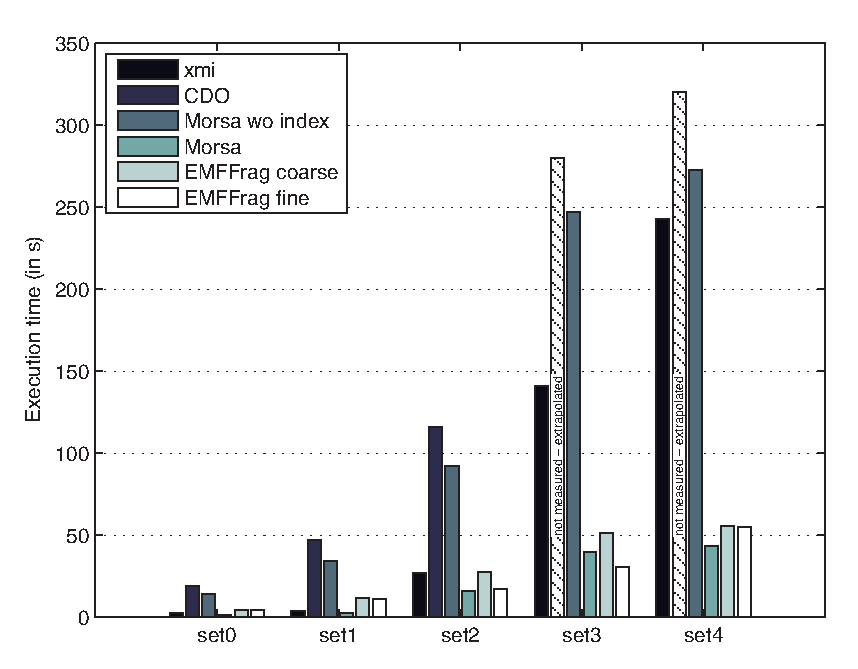
\includegraphics[width=\linewidth]{figures/grabatsQueryTimeExtra}
\caption{Execution time for querying the different Grabats models with the example query.}
\label{fig:grabatsQueryTime}
\end{minipage}
%\end{figure}
%\begin{figure}[ht]
\begin{minipage}[b]{0.48\linewidth}
\centering
\vspace{0.04\linewidth}
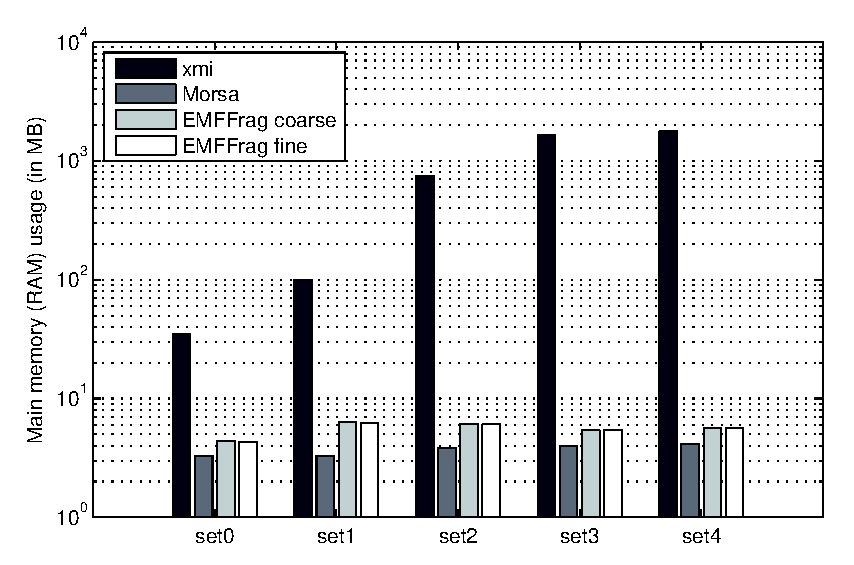
\includegraphics[width=\linewidth]{figures/grabatsTraverseMem}
\caption{Memory usage time for traversing the different Grabats.}
\label{fig:grabatsTraverseMem}
\end{minipage}
\hspace{0.02\linewidth}
\begin{minipage}[b]{0.48\linewidth}
\centering
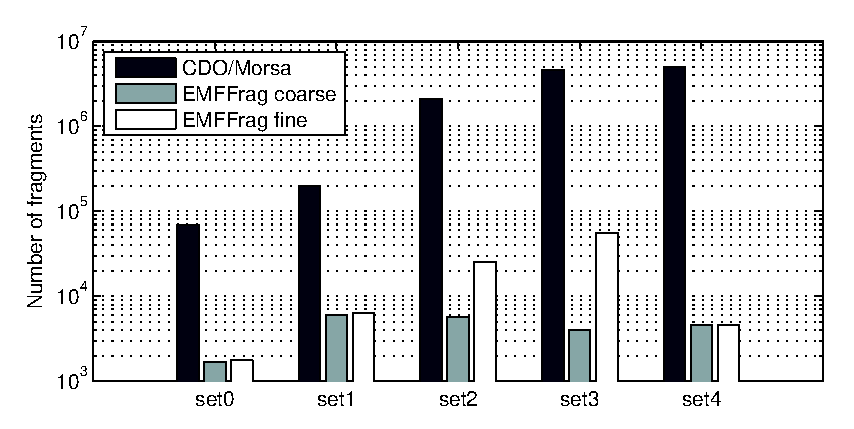
\includegraphics[width=\linewidth]{figures/grabatsFragments}
\caption{Number of fragments used by the different persistence solutions.}
\label{fig:grabatsFragments}
\end{minipage}
\end{figure}

The evaluation models are taken from the Grabats 2009 contest\markus{reference and some words}. There are five different software models. All covering Java projects. The models include the project structure, type structure, down to AST models of Java code. The five models have different sizes and complexities. Fig.~\ref{fig:grabatsFragments} shows the number of fragments that the different approaches used. Where EMF/XMI always uses only one fragment and morsa one fragment per object (i.e. the number of fragment equals the size of the model in number of objects). For EMFFrag, we used two differently strong fragmentations. First (Frag1), each class and compilation unit is put into a single fragment, and secondly (Frag2), additionally each method block is put in its own fragment. This shows the internal structure of sets zero through four: sets zero and one are pretty small, sets two and three containing lots of methods and its implementations, where set four seems to only contain information about projects, types, and members, but no implementation of members.

\subsubsection*{Model creation time}

\subsubsection*{Memory usage}

We measured the memory usage, needed for a full model access; the results are shown in Fig.~\ref{fig:grabatsLoadTraverseMem}. EMF/XMI's memory usage is proportional to model size, because it needs to load full models into memory. All other approaches need constant quantity of memory independent of model size. This quantity varies between the approaches, but is of an practical amount for all approaches. 

\subsubsection*{Full model access}

The execution times for accessing the complete models are shown in Fig.~\ref{fig:grabatsLoadTraverse}. Fist of all,  because the whole model is accessed, the execution time for all approaches grows with model size. EMF/XMI execution time grows more then linear due to pointless garbage collection. Morsa also shows sub linear performance, since each object has to be accessed individual, and even the best index only performs logarithmically depending on model size. EMFFrag performance is proportional to model size and number of fragments; as expected it takes longer to access the whole model on a more fragmented store.

\subsubsection*{Selective model access}

In this section, we present the execution times of model queries. The query is also taken from the grabats 2009 contest. The query is to find those \emph{TypeDeclaration} instances in the Java model that contain a static method with the containing type as return type. Morsa can profit from its index on the objects meta-class to find all instances of \emph{TypeDeclaration}. All other approaches have to traverse the model to find all instances of \emph{TypeDeclations}. For the Morsa approach, we used two implementations of the query: one using the meta-class index, and the other traversing the model as in all other approaches. The results are shown in Fig.~\ref{fig:grabatsQuery}.

\markus{TODO explain the query}


\subsection{The Influence of Fragmentation on Performance}

\begin{figure}
  \centering
  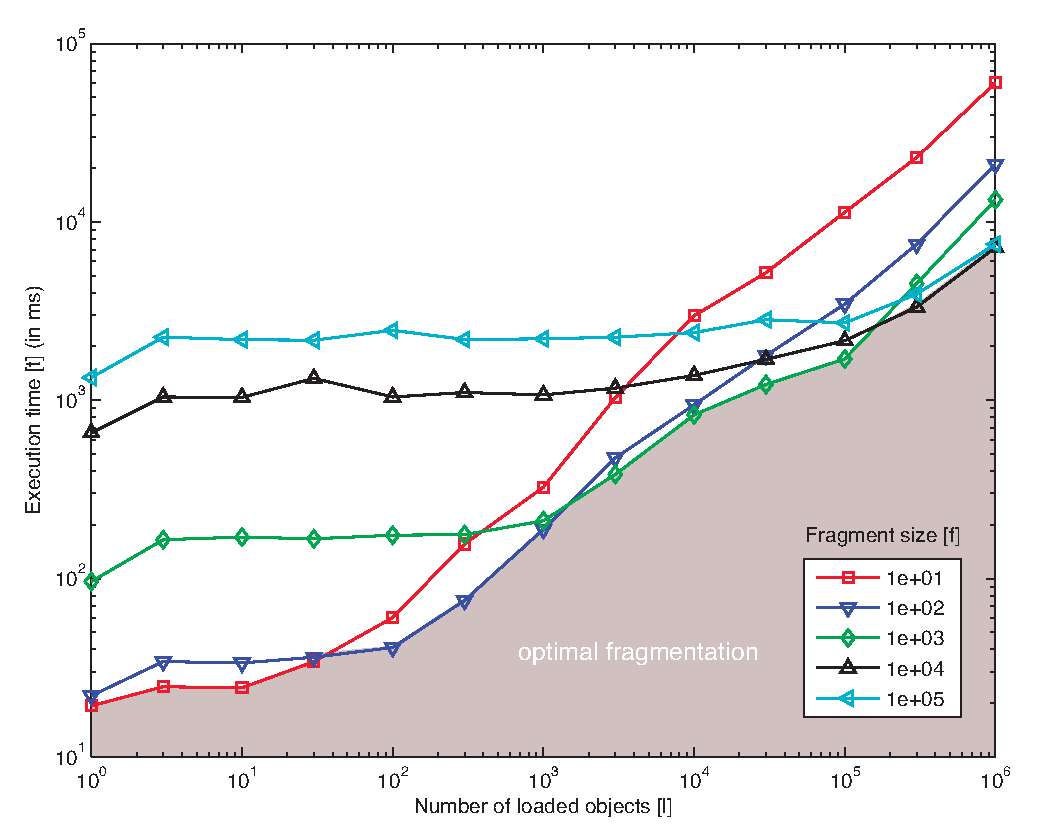
\includegraphics[width=0.65\linewidth]{figures/measureTimesExtra}
  \caption{Execution times for loading model parts with different fragmentation granularities.}
  \label{fig:measureTimeExtra}
\end{figure}

In this section, we look hat query and full access execution times for models of the same size and characteristics, but with different fragmentations. For this purpose, we use a simple meta-model (ref. to Fig.~\ref{?}). We generated models with a simple algorithm that takes model size, fragment size, and a so called \emph{depth factor} as parameters. The \emph{depth factor} determines the proportion of average number of object children to the overall model size, i.e. the depth of the model. 